\section{Versuchsaufbau}
\label{sec:aufbau}

\begin{figure}[H]
\begin{center}
  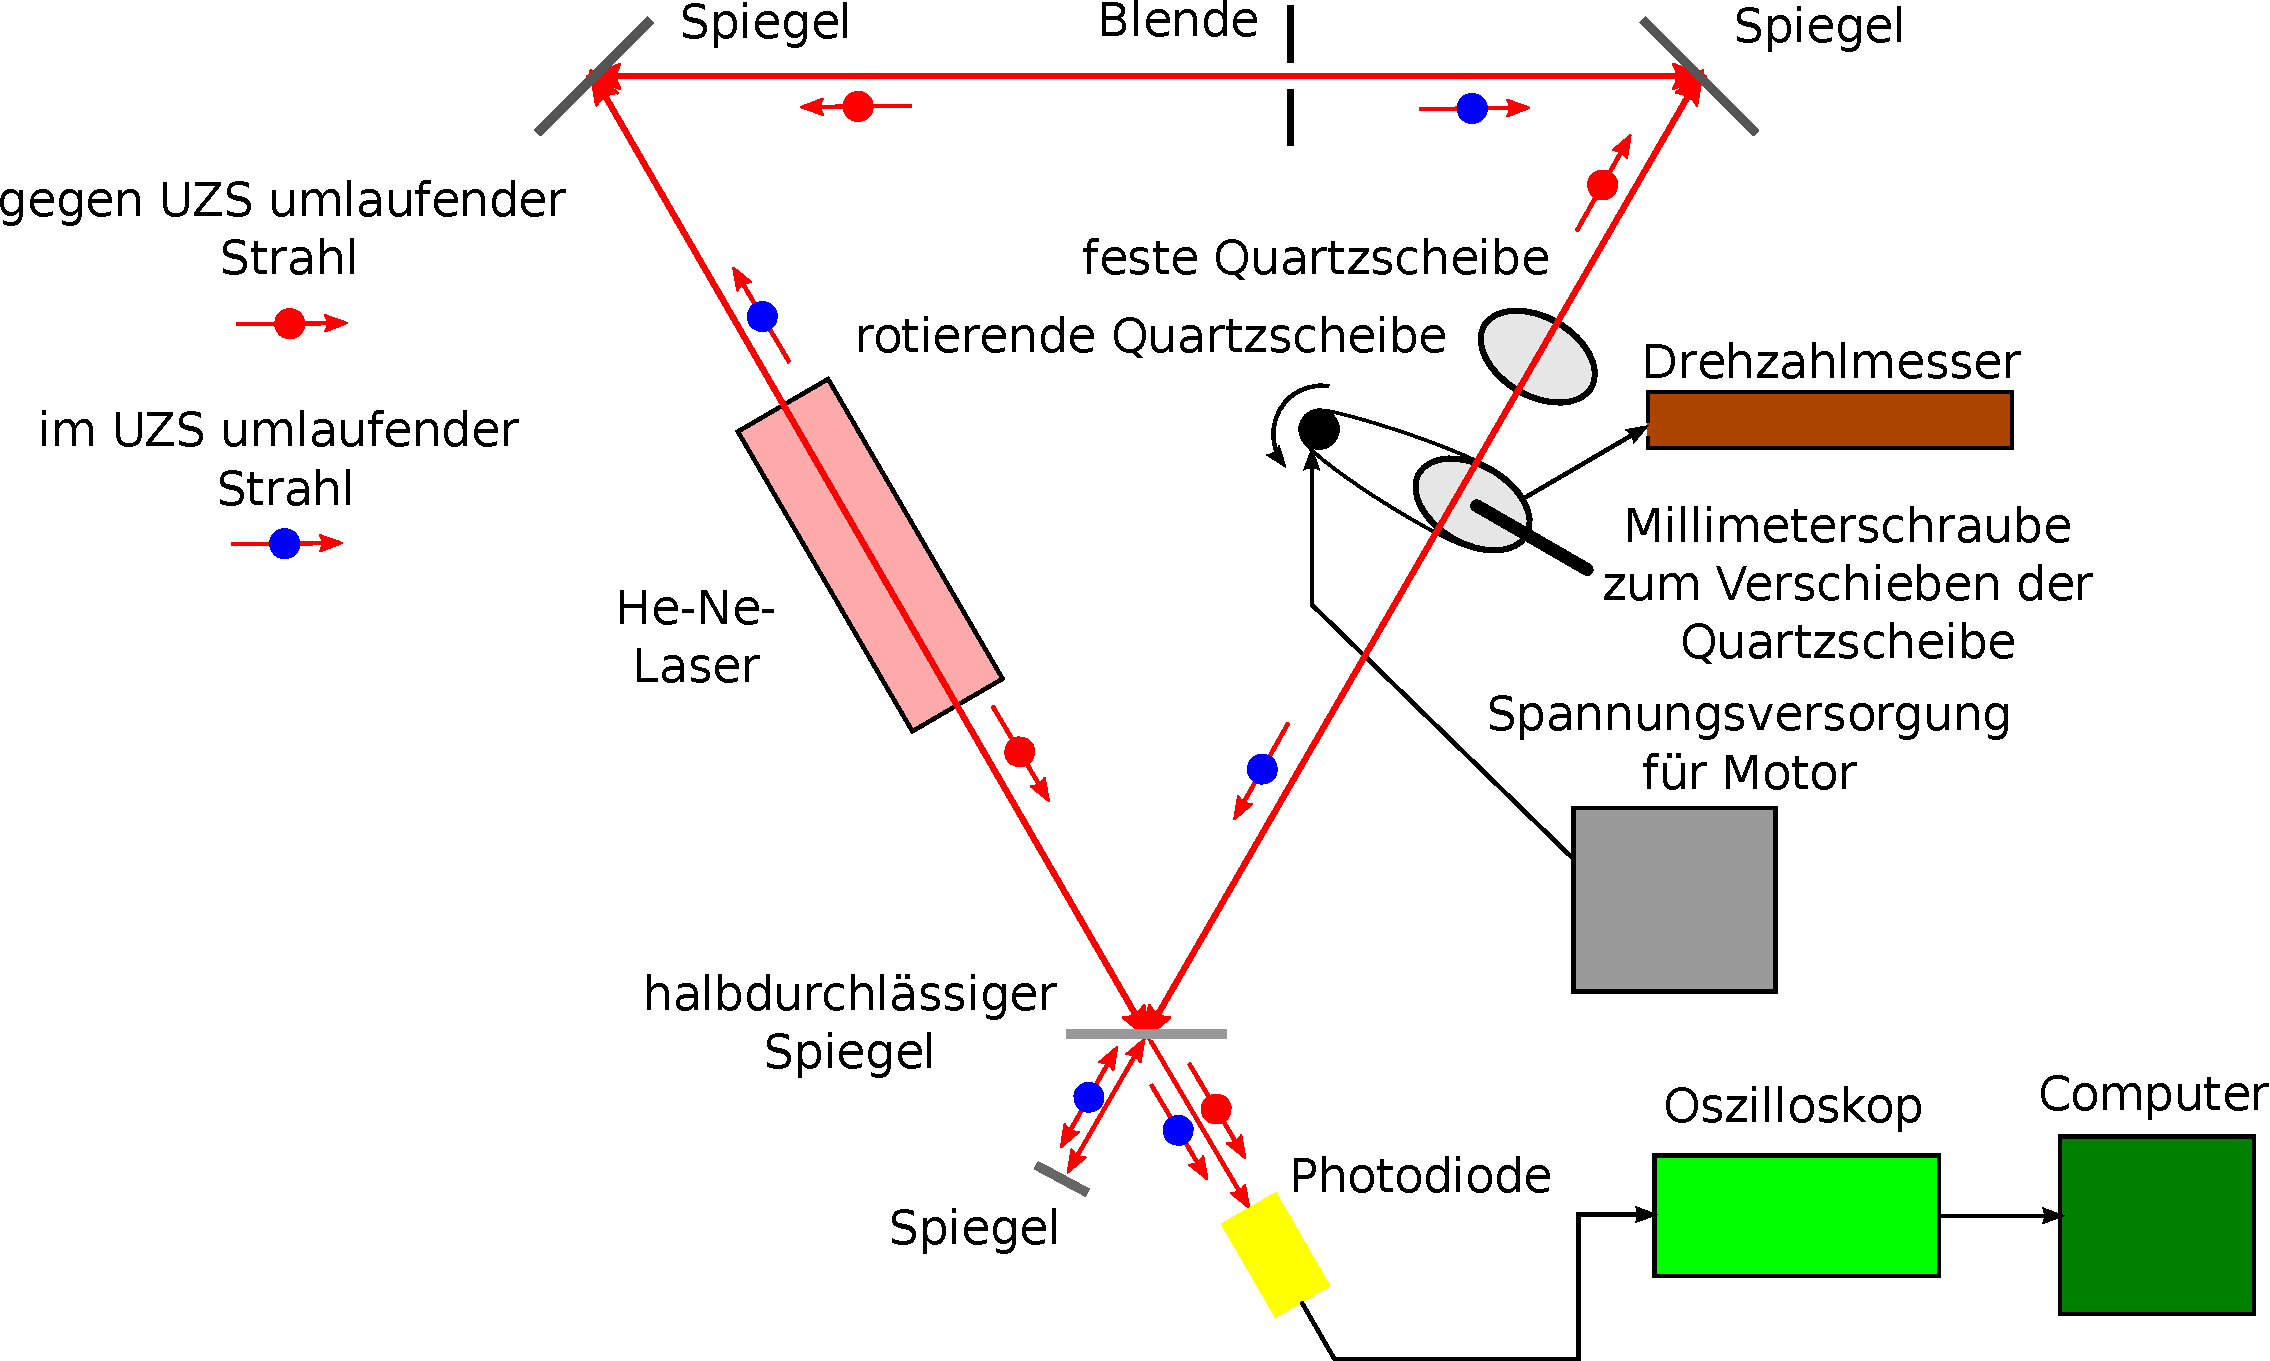
\includegraphics[width=0.95\textwidth]{../img/aufbau.pdf}
  \caption{Aufbau zur Bestimmung des Mitführungskoeffizinenten von Quarz mit einem Ringlaser.}
  \label{img:aufbau}
\end{center}
\end{figure}
\autoref{img:aufbau} zeigt den Aufbau des Ringlasers,
mit dem die Messungen durchgeführt werden.
Um eine Helium-Neon-Röhre,
die von einem statischen elektrischen Feld gepumpt wird,
ist mit drei Spiegeln ein Resonator aufgebaut.
Einer der Spiegel ist halbdurchlässig, um den Laserstrahl auszukoppeln.
Ein vierter Spiegel reflektiert den im Uhrzeigersinn umlaufenden Stahl so,
dass er zusammen mit dem anderen auf eine Photodiode fällt.
Der vierte Spiegel und der Halbdurchlässige können in ihrer Position verändert werden.
Im Strahlengang befindet sich außerdem eine einstellbare Blende,
mit der der Strahl abgeschwächt werden kann.
Zusätzlich sind im Strahlengang zwei Quarzscheiben,
die im Brewsterwinkel vom Laserstrahl getroffen werden.
Eine davon kann mit einem Motor in Rotation versetzt und ihre Drehzahl gemessen werden.
Die zweite, ruhende Scheibe ist dazu da,
den abgelenkten Strahl wieder zurück in den ursprünglichen Strahlverlauf zu brechen.\\
Das Signal der Photodiode wird auf einem Oszilloskop angezeigt und kann
vom Computer ausgelesen werden.